% Base sur la VO 0.11.9
% Relecture technique: 
% Relecture syntaxique: 

\part{Résumé des Règles}

\begin{table}[h!]
\begin{minipage}[t]{.35\linewidth}
\footnotesize

\subsubsection*{Tour de joueur}

\noindent
\begin{tabular}{c|m{4.5cm}}
\textbf{1} & Phase de Mouvement. \tabularnewline
\textbf{2} & Phase de Magie. \tabularnewline
\textbf{3} & Phase de Tir. \tabularnewline
\textbf{4} & Phase de Corps à corps. \tabularnewline
\end{tabular}

\smallskip

\subsubsection*{Étapes de la préparation}

\noindent
\begin{tabular}{c|m{4.5cm}}
\textbf{1} & Décidez de la taille de la partie. \tabularnewline
\textbf{2} & Montrez-vous vos listes d'armée. \tabularnewline
\textbf{3} & Décorez le champ de bataille. \tabularnewline
\textbf{4} & Déterminez le type de déploiement. \tabularnewline
\textbf{5} & Choisissez les objectifs secondaires. \tabularnewline
\textbf{6} & Déterminez les zones de déploiement. \tabularnewline
\textbf{7} & Générez les sorts. \tabularnewline
\textbf{8} & Déployez-vous. \tabularnewline
\end{tabular}

\smallskip

\subsubsection*{Étapes du déploiement}

\begin{tabular}{c|m{4.5cm}}
\textbf{1} & Déterminez qui commence à se déployer. \tabularnewline
\textbf{2} & Déployez des unités chacun votre tour. \tabularnewline
\textbf{3} & Déterminez qui va essayer d'avoir le premier tour. \tabularnewline
\textbf{4} & Déployez les unités restantes. \tabularnewline
\textbf{5} & Déployez les Éclaireurs. \tabularnewline
\textbf{6} & Déplacez les unités d'\emph{Avant-Garde}. \tabularnewline
\textbf{7} & Autres règles et capacités. \tabularnewline
\textbf{8} & Lancez le dé pour le premier tour. \tabularnewline
\end{tabular}

\end{minipage}
\hfill
\begin{minipage}[t]{.6\linewidth}
\footnotesize

\subsubsection*{Phase de Mouvement}

\noindent
\begin{tabular}{c|m{8.4cm}}
\textbf{1} & Début de la \emph{Phase de Mouvement}. \tabularnewline
\textbf{2} & Début de la sous-phase de déclaration des \emph{Charges}. \tabularnewline
\textbf{3} & Le joueur actif déclare ses \emph{Charges}. Il désigne les unités qui tentent de charger une unité ennemie. Pour chaque charge ainsi déclarée, le joueur réactif annonce la \emph{Réaction à charge} de son unité. \tabularnewline
\textbf{4} & Une fois que toutes les charges ont été déclarées, les unités en charge vont se déplacer. Le joueur actif lance maintenant les dés pour déterminer ses \emph{Jets de Charge}.\tabularnewline
\textbf{5} & Si une unité en charge ne parvient pas à atteindre sa cible, elle doit faire un \emph{Mouvement de charge ratée}.\tabularnewline
\textbf{6} & Si des unités en charge font un jet de dé suffisant pour charger, le joueur actif doit bouger ses unités et les aligner contre leur ennemi en maximisant le nombre de figurines au contact. L'unité en charge et l'unité chargée sont maintenant bloquées au corps à corps.\tabularnewline
\textbf{7} & Fin de la sous-phase de déclaration des \emph{Charges}. \tabularnewline
\textbf{8} & Début de la sous-phase des \emph{Mouvements Obligatoires}. \tabularnewline
\textbf{9} & Le joueur actif peut tenter de rallier ses troupes en fuite en effectuant ses \emph{Tests de ralliement}. \tabularnewline
\textbf{10} & Les unités n'ayant pas été ralliées (ou ne pouvant pas l'être) effectuent leur \emph{Mouvement de fuite}. \tabularnewline
\textbf{11} & Les unités possédant une caractéristique de mouvement aléatoire ou celles qui doivent faire un \emph{Mouvement obligatoire} se déplacent durant cette sous-phase. \tabularnewline
\textbf{12} & Fin de la sous-phase des \emph{Mouvements Obligatoires}. \tabularnewline
\textbf{13} & Début de la sous-phase des \emph{Autres Mouvements}. \tabularnewline
\textbf{14} & Le joueur actif déplace ses unités qui n'ont pas encore été déplacées.  (en effectuant des mouvements, des marches forcées ou des reformations). \tabularnewline
\textbf{15} & Fin de la sous-phase des \emph{Autres Mouvements}. \tabularnewline
\textbf{16} & Fin de la \emph{Phase de Mouvement}. \tabularnewline
\end{tabular}

\smallskip

\begin{tabular}{|m{9.5cm}|}
\hline
\textbf{Tests de Terrain Dangereux}
\newline Lancez un nombre de dés déterminé par le type de troupes de l'unité.
\newline Terrain dangereux (1) - le test est raté sur un \result{1}
\newline Terrain dangereux (2) - le test est raté sur un \result{1} ou \result{2}
\newline Terrain dangereux (3) - le test est raté sur un \result{1}, \result{2} ou \result{3}
\newline Pour chaque échec: l'unité subit une blessure avec \emph{Perforant (6)}.
\tabularnewline
\hline
\end{tabular}

\end{minipage}
\end{table}

\newpage
\begin{table}[h!]
\begin{minipage}[t]{.5\linewidth}
\footnotesize

\subsubsection*{Phase de Magie}

\begin{tabular}{c|m{6.8cm}}
\textbf{1} & Début de la \emph{Phase de Magie}. Lancez les dés pour déterminer les flux magiques et pour les canalisations. \tabularnewline
\textbf{2} & Les deux joueurs peuvent tenter de dissiper les sorts \emph{Reste en Jeu} lancés lors des phases de magie précédentes. \tabularnewline
\textbf{3} & Le joueur actif peut tenter de lancer ses sorts. \tabularnewline
\textbf{4} & Répétez les étapes 2 et 3 jusqu'à ce qu'aucun joueur ne fasse une action. \tabularnewline
\textbf{5} & Fin de la \emph{Phase de Magie}. Les capacités prenant effet à la fin de la \emph{Phase de Magie} sont déclenchées. \tabularnewline
\end{tabular}

\subsubsection*{Lancement d'un sort}

\begin{tabular}{c|m{6.8cm}}
\textbf{1} & Le joueur actif indique quel \emph{Sorcier} tente de lancer quel sort. Il doit préciser s'il opte pour une version améliorée du sort, ainsi que la cible du sort et de celle de l'attribut si nécessaire. Il indique aussi le nombre de dés de pouvoir utilisés (entre 1 et 5). \tabularnewline
\textbf{2} & Le joueur actif lance le nombre de dés de pouvoir annoncé, en les retirant de sa réserve. Additionnez les résultats des dés avec les modificateurs de lancer (tels qu'un \emph{Pouvoir irrésistible}). \tabularnewline
\textbf{3} & Le sort est lancé avec succès si le total de lancer est supérieur ou égal à la valeur de lancement. Sinon, le lancement de sort échoue et le lanceur subit l'effet \emph{Perte de Concentration}. \tabularnewline
\end{tabular}

\subsubsection*{Dissipation d'un sort}

\begin{tabular}{c|m{6.8cm}}
\textbf{1} & Le joueur réactif peut tenter de dissiper le sort. Dans ce cas, il doit indiquer lequel de ses \emph{Sorciers} n'étant pas en fuite (s'il en a) va tenter la dissipation, et annoncer combien de dés de dissipation il va utiliser (un minimum d' un dé est nécessaire, et la totalité de réserve peut être utilisée). Il est possible de tenter une dissipation même sans avoir de \emph{Sorcier}. \tabularnewline
\textbf{2} & Le joueur réactif lance le nombre de dés de dissipation annoncé, en les retirant de sa réserve. Additionnez les résultats des dés avec les modificateurs de dissipation (tels qu'un \emph{Pouvoir irrésistible}) pour obtenir le total de dissipation. \tabularnewline
\textbf{3} & Si le résultat est supérieur ou égal au total de lancement, le sort est dissipé, et le lancement du sort a échoué. Sinon, le \emph{Sorcier} ayant tenté la dissipation subit l'effet \emph{Perte de Concentration}. \tabularnewline
\end{tabular}

\end{minipage}
\hfill
\begin{minipage}[t]{.5\linewidth}
\footnotesize

\subsubsection*{Tableau des Fiascos}

\begin{tabular}{cm{6.8cm}}
\hline
\textbf{2 à 4} & Centrez le gabarit de 5{\pouce} sur le lanceur. Toute figurine recouverte par le gabarit, même partiellement, subit une touche. De plus, si NDP = \textbf{5}, retirez le lanceur de la partie. Si NDP = 4, lancez un D6. Sur un résultat de 1 à 3, le lanceur est retiré de la partie. \tabularnewline
\textbf{5 à 6} & Centrez le gabarit de 3{\pouce} sur le lanceur. Toute figurine recouverte par le gabarit subit une touche. Le lanceur doit subir une touche. \tabularnewline
\textbf{7} & L'unité du lanceur subit NDP touches, réparties comme des tirs. Le lanceur ne peut cependant subir qu'une seule touche au maximum. \tabularnewline
\textbf{8 à 9} & Le lanceur et tout \emph{Sorcier} ami subissent une touche. \tabularnewline
\textbf{10 à 12} & Le niveau de magie du lanceur est diminué de NDP - 2. Il perd un sort pour chaque niveau de magie perdu, en commençant par le sort ayant causé le \emph{Fiasco} et en tirant les autres au hasard. \tabularnewline
\hline
\end{tabular}

\bigskip
Après le jet sur cette table, retirez NDP dés de votre réserve.
\smallskip

\begin{tabular}{|m{8cm}|}
\hline
\textbf{Modificateurs magiques}
\newline Sorcier de niveau 1 ou 2: Apprenti, +1
\newline Sorcier de niveau 3 ou 4: Maître, +2
\newline La somme des modificateurs ne peut pas dépasser +3, sauf en cas de \emph{Pouvoir Irrésistible} (ce dernier ajoute 1D3 + NDP). \tabularnewline
\hline
\end{tabular}

\bigskip

\begin{tabular}{|m{8cm}|}
\hline
\textbf{Objets de sorts}
\newline Pour lancer un objet de sort avec succès, le jet de lancement doit être supérieur ou égal à son niveau de puissance.
\smallskip
\begin{itemize}
\item Aucun modificateur positif ne peut être ajouté au jet de lancement.
\item Un échec de provoque pas de \emph{Perte de concentration} pour le lanceur.
\item Un objet de sort ne bénéficie pas du bonus de lancement d'un \emph{Pouvoir Irrésistible}.
\item L'attribut de la Discipline est lancé comme d'ordinaire.
\end{itemize}
En cas de \emph{Pouvoir Irrésistible}:
\begin{itemize}
\item Si 4 dés ou plus ont été utilisés pour lancer le sort, l'objet de sort est perdu et ne peut plus être lancé pendant la partie.
\item Retirez NDP dés de pouvoir de votre réserve.
\end{itemize}
\tabularnewline
\hline
\end{tabular}

\end{minipage}
\end{table}

\newpage
\begin{table}[h!]
\begin{minipage}[t]{.65\linewidth}
\footnotesize

\subsubsection*{Phase de tir}

\begin{tabular}{c|m{9.7cm}}
\textbf{1} & Le joueur actif choisit une unité avec laquelle tirer et désigne l'unité ennemie visée. \tabularnewline
\textbf{2} & Le joueur actif mesure la distance entre son unité et l'unité ennemie visée pour être sûr que celle-ci est bien à portée de tir. Il doit aussi s'assurer que son unité a une ligne de vue sur l'unité visée.\tabularnewline
\textbf{3} & Le joueur actif effectue ses jets pour toucher en tenant compte des \emph{Modificateurs de tir}. \tabularnewline
\textbf{4} & Pour chaque touche réussie, le joueur actif effectue ses jets pour blesser. \tabularnewline
\textbf{5} & Pour chaque blessure subie, le joueur réactif effectue ses sauvegardes d'armures, sauvegardes invulnérables et autres jets de \emph{Régénération}. \tabularnewline
\textbf{6} & Le joueur réactif retire ses pertes pour chaque blessure infligée. Notez les points de vie perdus pour les figurines ayant plusieurs points de vie. \tabularnewline
\textbf{7} & Le joueur actif choisit une nouvelle unité qui n'a pas tiré lors de cette phase et répète les étapes de 1 à 6. \tabularnewline
\textbf{8} & Dès qu'une unité subit de \emph{Lourdes pertes} (perte de 25\% ou plus de l'effectif en début de phase), elle effectue un test de \emph{Panique}. \tabularnewline
\textbf{9} & La \emph{Phase de Tir} prend fin. \tabularnewline
\end{tabular}

\smallskip

\subsubsection*{Tableau des Incidents de Tir}

\begin{tabular}{c m{8cm}}
\hline
Résultat & Effet \tabularnewline
\result{0} ou moins & \textbf{Explosion!} \newline Toutes les figurines à moins de 1D6{\pouce} de la figurine qui subit un \emph{Incident de Tir} reçoivent une touche de Force 5. La figurine qui tire est détruite, retirez-la comme perte. \tabularnewline
1 à 2 & \textbf{Défaillance critique} \newline Le mécanisme de tir est endommagé. La figurine ne peut plus tirer avec cette arme pour le restant de la partie. \tabularnewline
3 à 4 & \textbf{Enrayé} \newline Cette \emph{Arme d'Artillerie} ne peut pas être utilisée au prochain tour de son propriétaire. \tabularnewline
5+ & \textbf{Dysfonctionnement} \newline La figurine subit une blessure sans sauvegarde d'aucune sorte autorisée. \tabularnewline
\hline
\end{tabular}

\end{minipage}
\hfill
\begin{minipage}[t]{.3\linewidth}
\footnotesize

\subsubsection*{Jets pour toucher au tir}

\begin{tabular}{cc}
\hline
\textbf{CT + modif.} & \textbf{Résultat nécessaire} \\
6 ou plus & 2+ \\
5 & 2+ \\
4 & 3+ \\
3 & 4+ \\
2 & 5+ \\
1 & \result{6} \\
0 & \result{6} suivi par 4+ \\
-1 & \result{6} suivi par 5+ \\
-2 & \result{6} suivi d'un \result{6} \\
-3 ou moins & impossible \\
\hline
\end{tabular}

\bigskip

\subsubsection*{Modificateurs des jets pour toucher au tir}

\begin{tabular}{r|c}
Longue portée & -1 \\
Bouger et tirer & -1 \\
Tenir la position et tirer & -1 \\
Couvert léger & -1 \\
Couvert lourd & -2 \\
\end{tabular}

\smallskip

\subsubsection*{Distribution des attaques}

\begin{tabular}{c|m{5cm}}
\textbf{1} & L'attaquant distribue les touches. \tabularnewline
\textbf{2} & L'attaquant fait les jets pour blesser. \tabularnewline
\textbf{3} & Sauvegardes d'armure. \tabularnewline
\textbf{4} & Sauvegardes spéciales. \tabularnewline
\textbf{5} & Le défenseur retire ses pertes ou marque les blessures subies. \tabularnewline
\textbf{6} & Test de \emph{Panique} éventuel. \tabularnewline
\end{tabular}

\end{minipage}
\end{table}

\subsubsection*{Lignes de vues et couverts}
\begin{center}
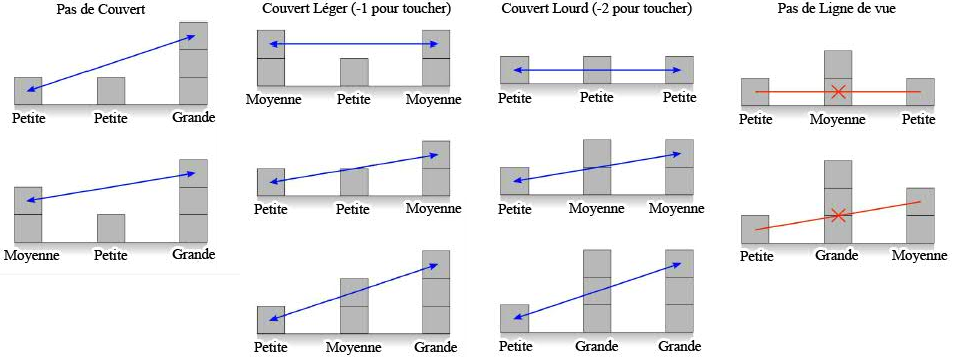
\includegraphics[width=13cm]{Lignes_de_vue2.png}
\end{center}

\newpage

\begin{table}[h!]
\begin{minipage}[t]{.4\linewidth}
\footnotesize

\subsubsection*{Phase de corps à corps}

\begin{tabular}{c|m{6cm}}
\textbf{1} & Début de la \emph{Phase de Corps à Corps}. Appliquez la règle \emph{Plus Engagés} si nécessaire. \tabularnewline
\textbf{2} & Choisissez un combat. \tabularnewline
\textbf{3} & Résolvez ce combat pour cette phase. \tabularnewline
\textbf{4} & Répétez les étapes 2 et 3 pour chaque combat qui n'a pas encore eu lieu pendant cette phase. \tabularnewline
\textbf{5} & Quand toutes les unités engagées au corps à corps ont combattu, la \emph{Phase de Corps à Corps} prend fin. \tabularnewline
\end{tabular}

\bigskip

\subsubsection*{Résumé du résultat de combat}
\begin{tabular}{l m{3.5cm}}
\hline
Blessures infligées & +1 par blessure \tabularnewline
Carnage & +1 par blessure (max \nouveau{+3}) \tabularnewline
Charge & +1 (+2 depuis une colline) \tabularnewline
Bonus de rang & +1 par rang (max +3) \tabularnewline
Étendard & +1 \tabularnewline
Grande bannière & +1 \tabularnewline
Bonus de flanc & +1 \nouveau{ou +2} \tabularnewline
Bonus d'arriere & +1 \nouveau{ou +2} \tabularnewline
\hline
\end{tabular}

\end{minipage}
\hfill
\begin{minipage}[t]{.55\linewidth}
\footnotesize

\subsubsection*{Étapes d'une manche de corps à corps}

\begin{tabular}{c|m{8cm}}
\textbf{1} & Début de la manche de corps à corps. \tabularnewline
\textbf{2} & Choisissez les armes que vos unités utilisent. \tabularnewline
\textbf{3} & Les personnages peuvent faire un mouvement en suivant la règle \emph{Faites Place}. \tabularnewline
\textbf{4} & Lancez et relevez ou refusez les \emph{Défis}. \tabularnewline
\textbf{5} & Faites les attaques, par ordre d'Initiative:
\newline - Allouez les attaques.
\newline - Lancez les jets pour toucher, pour blesser, les jets de sauvegarde et retirez les pertes.
\newline - Passez à l'étape d'Initiative suivante. \tabularnewline
\textbf{6} & Le ou les perdants font un test de \emph{Moral}. Une unité qui rate son test de \emph{Moral} prend la \emph{Fuite}. Si aucune unité ne fuit, passez à l'étape 11. \tabularnewline
\textbf{7} & Effectuez les tests de \emph{Panique} pour les unités proches des unités qui ont raté leur test de \emph{Moral}. \tabularnewline
\textbf{8} & Si une unité prend la \emph{Fuite}, le vainqueur choisit de poursuivre ou non. S'il veut \emph{Réfréner sa poursuite}, un test de Commandement doit être effectué. \tabularnewline
\textbf{9} & Jet des distances de fuite et déplacement des unités en fuite. \tabularnewline
\textbf{10} & Jet des distances de poursuite et déplacement des unités poursuivantes. \tabularnewline
\textbf{11} & Effectuez les \emph{Pivots Post-Combat}. \tabularnewline
\textbf{12} & Effectuez les \emph{Reformations de Combat}. \tabularnewline
\textbf{13} & Fin de la manche de corps à corps. Passez au combat suivant. \tabularnewline
\end{tabular}

\end{minipage}
\end{table}

\begin{table}[h!]
\begin{minipage}[t]{.5\linewidth}
\footnotesize

\subsubsection*{Jets pour toucher au corps à corps}

\begin{tabular}{c|m{.2cm}m{.2cm}m{.2cm}m{.2cm}m{.2cm}m{.2cm}m{.2cm}m{.2cm}m{.2cm}m{.2cm}}
\backslashbox{D}{A} & \centering 1 & \centering 2 & \centering 3 & \centering 4 & \centering 5 & \centering 6 & \centering 7 & \centering 8 & \centering 9 & 10 \\
\hline
1 & \yel 4+ & \lem 3+ & \lem 3+ & \lem 3+ & \lem 3+ & \lem 3+ & \lem 3+ & \lem 3+ & \lem 3+ & \lem 3+ \\
2 & \yel 4+ & \yel 4+ & \lem 3+ & \lem 3+ & \lem 3+ & \lem 3+ & \lem 3+ & \lem 3+ & \lem 3+ & \lem 3+ \\
3 & \ora 5+ & \yel 4+ & \yel 4+ & \lem 3+ & \lem 3+ & \lem 3+ & \lem 3+ & \lem 3+ & \lem 3+ & \lem 3+ \\
4 & \ora 5+ & \yel 4+ & \yel 4+ & \yel 4+ & \lem 3+ & \lem 3+ & \lem 3+ & \lem 3+ & \lem 3+ & \lem 3+ \\
5 & \ora 5+ & \ora 5+ & \yel 4+ & \yel 4+ & \yel 4+ & \lem 3+ & \lem 3+ & \lem 3+ & \lem 3+ & \lem 3+ \\
6 & \ora 5+ & \ora 5+ & \yel 4+ & \yel 4+ & \yel 4+ & \yel 4+ & \lem 3+ & \lem 3+ & \lem 3+ & \lem 3+ \\
7 & \ora 5+ & \ora 5+ & \ora 5+ & \yel 4+ & \yel 4+ & \yel 4+ & \yel 4+ & \lem 3+ & \lem 3+ & \lem 3+ \\
8 & \ora 5+ & \ora 5+ & \ora 5+ & \yel 4+ & \yel 4+ & \yel 4+ & \yel 4+ & \yel 4+ & \lem 3+ & \lem 3+ \\
9 & \ora 5+ & \ora 5+ & \ora 5+ & \ora 5+ & \yel 4+ & \yel 4+ & \yel 4+ & \yel 4+ & \yel 4+ & \lem 3+ \\
10 & \ora 5+ & \ora 5+ & \ora 5+ & \ora 5+ & \yel 4+ & \yel 4+ & \yel 4+ & \yel 4+ & \yel 4+ & \yel 4+ \\
\end{tabular}

\end{minipage}
\hfill
\begin{minipage}[t]{.5\linewidth}
\footnotesize

\subsubsection*{Jets pour blesser}

\begin{tabular}{c|m{.2cm}m{.2cm}m{.2cm}m{.2cm}m{.2cm}m{.2cm}m{.2cm}m{.2cm}m{.2cm}m{.2cm}}
\backslashbox{E}{F} & 1 & 2 & 3 & 4 & 5 & 6 & 7 & 8 & 9 & 10 \\
\hline
1 & \yel 4+ & \lem 3+ & \gre 2+ & \gre 2+ & \gre 2+ & \gre 2+ & \gre 2+ & \gre 2+ & \gre 2+ & \gre 2+ \\
2 & \ora 5+ & \yel 4+ & \lem 3+ & \gre 2+ & \gre 2+ & \gre 2+ & \gre 2+ & \gre 2+ & \gre 2+ & \gre 2+ \\
3 & \red 6+ & \ora 5+ & \yel 4+ & \lem 3+ & \gre 2+ & \gre 2+ & \gre 2+ & \gre 2+ & \gre 2+ & \gre 2+ \\
4 & \red 6+ & \red 6+ & \ora 5+ & \yel 4+ & \lem 3+ & \gre 2+ & \gre 2+ & \gre 2+ & \gre 2+ & \gre 2+ \\
5 & \red 6+ & \red 6+ & \red 6+ & \ora 5+ & \yel 4+ & \lem 3+ & \gre 2+ & \gre 2+ & \gre 2+ & \gre 2+ \\
6 & \red 6+ & \red 6+ & \red 6+ & \red 6+ & \ora 5+ & \yel 4+ & \lem 3+ & \gre 2+ & \gre 2+ & \gre 2+ \\
7 & \red 6+ & \red 6+ & \red 6+ & \red 6+ & \red 6+ & \ora 5+ & \yel 4+ & \lem 3+ & \gre 2+ & \gre 2+ \\
8 & \red 6+ & \red 6+ & \red 6+ & \red 6+ & \red 6+ & \red 6+ & \ora 5+ & \yel 4+ & \lem 3+ & \gre 2+ \\
9 & \red 6+ & \red 6+ & \red 6+ & \red 6+ & \red 6+ & \red 6+ & \red 6+ & \ora 5+ & \yel 4+ & \lem 3+ \\
10 & \red 6+ & \red 6+ & \red 6+ & \red 6+ & \red 6+ & \red 6+ & \red 6+ & \red 6+ & \ora 5+ & \yel 4+ \\
\end{tabular}

\end{minipage}
\end{table}

\newpage

{
\footnotesize

{\normalsize \noindent \textbf{Résumé des différents types de troupes}}

\renewcommand{\arraystretch}{1.1}
\setlength{\tabcolsep}{2pt}
\noindent
\begin{tabular}{m{5cm}l}
RC (H) - Rang complet (horde)
&
TTD - Nombre de dés nécessaires pour les tests de terrain dangereux
\end{tabular}
\newline \noindent
\begin{tabular}{M{3.5cm}M{1.9cm}M{0.9cm}M{2.3cm}M{3.9cm}M{1.4cm}M{0.7cm}}
 & \textbf{Type de profil} & \textbf{RC (H)} & \textbf{Soutien} & \textbf{Règles spéciales} & \textbf{Taille**} & TTD \\
\rowcolor{lightgray!20} \textbf{Infanterie} & - & 5 (10) & 1 & - & Petite & 1 \\
\textbf{Bête de Guerre} & - & 5 (10) & 1 & \emph{Rapide} & Petite & 1 \\
\rowcolor{lightgray!20} \textbf{Cavalerie} & \emph{Profil Combiné} & 5 (10) & 1 (cavalier) & \emph{Rapide} & Moyenne & 1 \\
\textbf{Infanterie Monstrueuse} & - & 3 (6) & max 3 & \emph{Piétinement (1)} & Moyenne & 2 \\
\rowcolor{lightgray!20} \textbf{Bête Monstrueuse} & - & 3 (6) & max 3 & \emph{Piétinement (1)}, \emph{Rapide} & Moyenne & 2 \\
\textbf{Cavalerie Monstrueuse} & \emph{Profil Combiné} & 3 (6) & max 3 (cavalier) & \emph{Piétinement (1)}, \emph{Rapide} & Moyenne & 2 \\
\rowcolor{lightgray!20} \textbf{Char} & \emph{Profil Combiné} & 3 (6) & 1 (1 membre d'équipage) & \emph{Pas de Marche Forcée}, \emph{Rapide}, \emph{Touches d'Impact (1D6)} & Moyenne & 4 \\
\textbf{Monstre} & - & 1 & - & \emph{Grande Cible}, \emph{Piétinement (1D6)}, \emph{Terreur} & Grande & 4 \\
\rowcolor{lightgray!20} \textbf{Monstre Monté} & \emph{Profil de monstre monté} & 1 & - & \emph{Grande Cible}, \emph{Piétinement (1D6)}, \emph{Terreur} & Grande & 4 \\
\textbf{Nuée} & - & * (10) & 1 & \emph{Indémoralisable}, \emph{Instable}, \emph{Tirailleurs} & Petite & 1 \\
\rowcolor{lightgray!20} \textbf{Machine de Guerre} & \emph{Machine de Guerre} & Pas de rangs & - & \emph{Mouvement ou Tir}, \emph{Pas de Marche Forcée}, \emph{Tir Lent} & Petite & 1 \\
\end{tabular}
\newline * Les Nuées ne peuvent pas avoir de rang complet puisqu'elles ont la règle  \emph{Tirailleurs}
\newline ** Toutes les figurines qui ont la règle \emph{Grande Cible} sont de Grande taille.


\medskip
{\normalsize \noindent \textbf{Touches des Gabarits}}
\newline \noindent Nombre maximal de figurines pouvant être touchées par un gabarit. Socles verts: 20x20\milli\meter{}, socles roses: 25x25\milli\meter{}, socles bleu clair: 40x40\milli\meter{}, socles orange: 25x50\milli\meter{}. Un gabarit de ligne peut toucher plusieurs figurines par rang.
\begin{center}
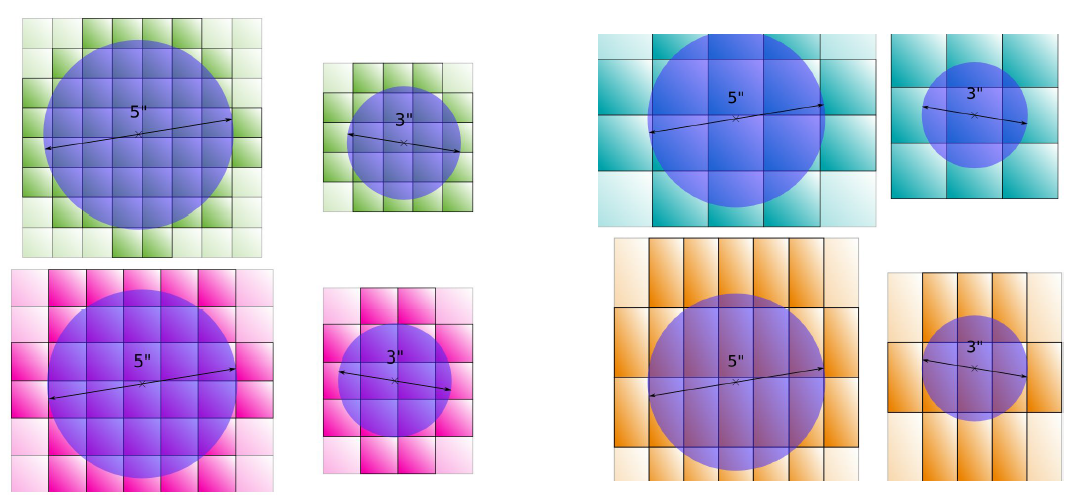
\includegraphics[width=7cm]{gabarits_1.png}
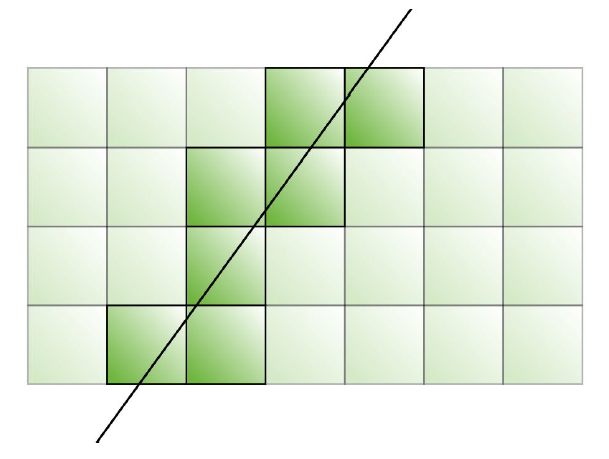
\includegraphics[width=4cm]{gabarits_2.png}
\end{center}

\renewcommand{\arraystretch}{1.1}
\noindent
\setlength{\tabcolsep}{2pt}
\begin{tabular}{m{5cm}l}
TD - Terrain dangereux
&
CCMC - Cavalerie, Cavalerie monstrueuse et Chars
\end{tabular}
\newline \noindent
\begin{tabular}{M{1.9cm}M{5cm}M{5.4cm}M{4.5cm}}
\textbf{Terrain} & \textbf{Mouvement} & \textbf{Couvert} & \textbf{Autre} \\
\rowcolor{lightgray!20} Terrain infranchissable & Distance minimale: 1\pouce \newline TD (3) pour les unités en fuite & Terrain occultant, couvert lourd & \\
Champs & TD(1) pour CCMC et les figurines avec des \emph{Attaques enflammées} & & Donne \emph{Inflammable} \\
\rowcolor{lightgray!20} Collines & & Terrain occultant \newline Unités partiellement sur la colline: couvert léger \newline Unités hors de la colline: couvert lourd & Donne \emph{Grande cible} \newline Charger depuis une colline donne +1 au résultat de combat \\
Forêts & TD (1) pour CCMC et les unités avec \emph{Vol} & Couvert léger & Pas d'\emph{Indomptable}. Donne \emph{Tenace} aux \emph{Tirailleurs} et aux personnages d'infanterie seuls. \\
\rowcolor{lightgray!20} Ruines & TD (1) pour toute unité non \emph{Tirailleurs} \newline TD (2) pour CCMC & Unités partiellement dans les ruines: couvert lourd, sauf \emph{Grandes cibles} & \\
Eaux peu profondes & TD (1) pour CCMC & & \emph{Désorganise} les rangs \\
\rowcolor{lightgray!20} Murs & Ignorez les murs pour le mouvement, sauf: TD(1) pour CCMC & Donne un couvert lourd et \emph{Distrayant} pour la première phase de combat, sauf \emph{Grande cible} & \\
\end{tabular}
%\renewcommand{\arraystretch}{1.5}
}